\newpage
\section{遊泳実験}
外皮の有無による遊泳性能への影響を検証するために,柔軟外皮未装着時と柔軟外皮装着時それぞれで直進遊泳実験を行った.

\subsection{実験条件}
実験においてはサーボモータにステップ状の入力を与え,ワイヤを断続的に左右に巻き取ることで胴体を振る動作を実現した(図\ref{fig:servo_seigyo}).$T$ [ms]は入力の周期,
$\theta$ [deg]はプーリの回転角(糸の巻き取り量)を表している.
遊泳実験ではこの周期から決定される尾ビレ周波数と,ワイヤの巻き取り量から決定される尾びれ振幅の2つをパラメータとした.尾びれ周波数は尾びれを振る頻度を決定するパラメータ
であり,$f = 1/T$ [Hz]で算出する.
\begin{figure}[hb]
    \centering
    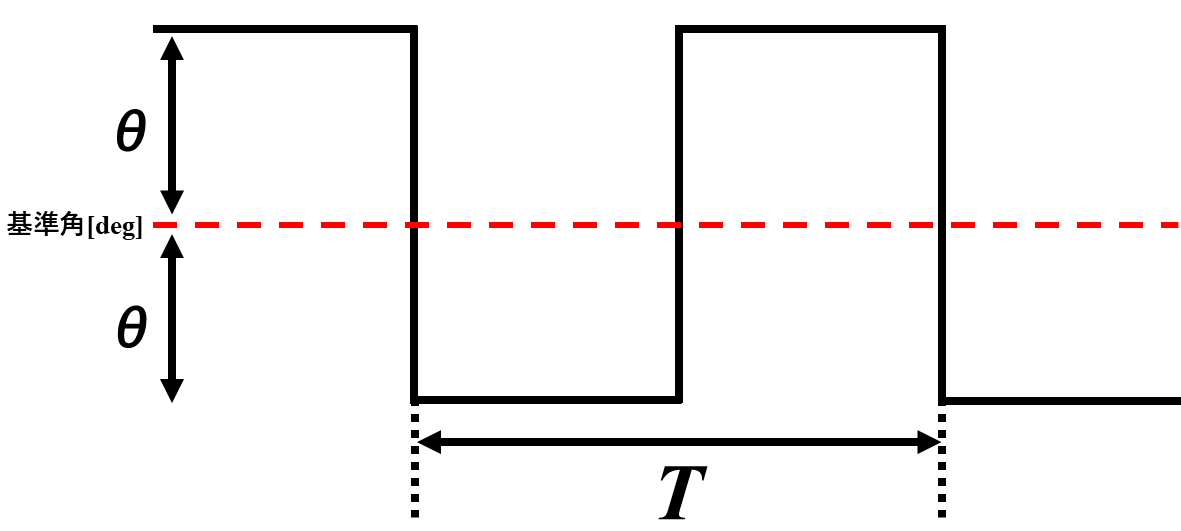
\includegraphics[width=0.75\linewidth]{chapters/picture/servo2.png}
    \caption{サーボへの制御入力}
    \label{fig:servo_seigyo}
\end{figure}
\begin{figure}[hb]
    \centering
    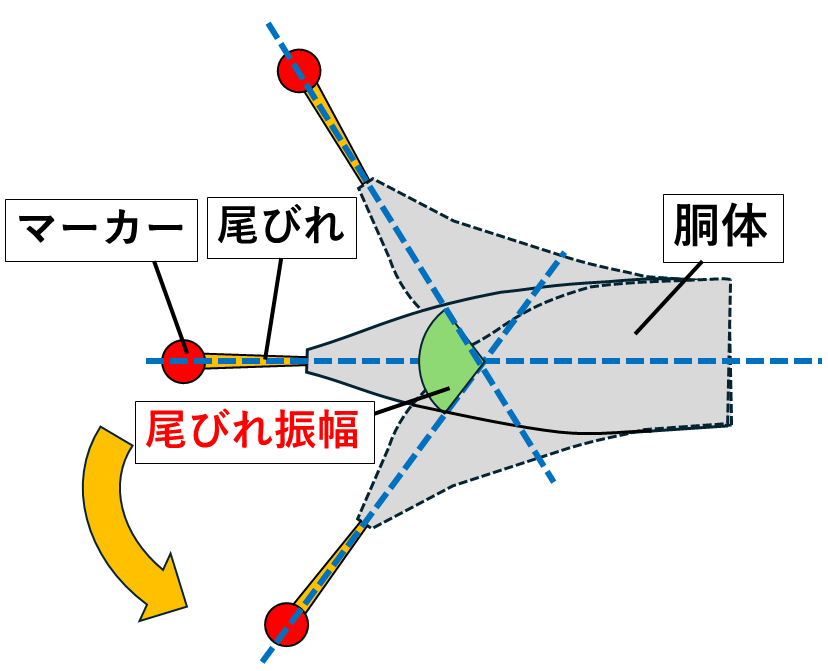
\includegraphics[width=0.6\linewidth]{chapters/picture/obire_amp.png}
    \caption{尾びれ振幅について}
    \label{fig:obire_amp}
\end{figure}
尾びれ振幅は体をどのくらい屈曲させるかのパラメータであり,ワイヤの巻き取り量が多いほど大きくなる(図\ref{fig:obire_amp}).柔軟外皮未装着の状態で,空中にて動作させた様子からトラッキングソフト
「kinovea」を用いて調べた結果,プーリの回転角が$30\:^\circ$,$45\:^\circ$,$60\:^\circ$のとき,尾びれ振幅はそれぞれ$81\:^\circ$,$114\:^\circ$,$168\:^\circ$であ
ったため,尾びれ振幅についてはこの3種類を実験に用いることとした. 

実験は直進遊泳とした.尾びれ振幅は$81\:^\circ$,$114\:^\circ$,$168\:^\circ$の3パターン,尾びれ周波数は0.5~1.75 Hzまで0.25 Hz刻みで6 パターン,さらに柔軟外皮の有無で2 パターン,合計36 
パターンのパラメータセットについて実験を行った.実験は各パラメータセットにつき3 回を行い,得られた遊泳速度のデータから平均,分散,標準偏差を算出した.
遊泳実験は室内に設置された1.5 m × 2.5 mのプールにて行い,その様子を天井に取り付けたカメラにて撮影を行った.その動画から,ロボット尾びれに取り付けたマーカーをkinoveaで
トラッキングして尾ビレ軌跡を取得する.
さらに尾びれ軌跡のトラッキングデータを二次近似し, 積分して遊泳距離を算出し,遊泳時間で除算して遊泳速度を算出する. なお遊泳開始直後
を過渡状態とみなし,遊泳速度は遊泳開始時点から500~1500 mmの範囲のデータを用いて算出した.

\subsection{実験結果}
図\ref{fig:test_swim}に柔軟外皮を装着した状態で尾びれ振幅$168\:^\circ$,尾びれ周波数1.75 Hzの時の遊泳実験の様子を示す.全ての遊泳実験において頭部に浸水することはなく,バッテリーの
交換やメンテンナンスなども試作機と比べてスムーズに行うことができた.また,柔軟外皮はリンクにうまく追従して遊泳し,胴体を屈曲させたときにしわがよることもなかった.しかし,遊泳
時の様子を見ると同じパラメータでも図\ref{fig:kukkyoku}のように柔軟外皮装着時に尾びれの振りの大きさが未装着時よりも小さくなる傾向があった.また,すべての遊泳実験で図\ref{fig:str}のように直進させたかったが,
図\ref{fig:right}のように進行方向が右に傾いたり左に傾いたりしてしまう時があった.

次に実験結果から遊泳速度を計測した結果を図\ref{fig:amp}に示す.グラフのエラーバーは標準偏差を示している.グラフから,まず柔軟外皮あり・なし両方に共通して尾びれ周波数が
高くなるほど遊泳速度が大きくなっていることがわかる.また,すべての実験において柔軟外皮装着状態の方が未装着時よりも遊泳速度が速くなっている.さらに尾びれ振幅が大きくなるにつれて
柔軟外皮装着時と未装着時における速度差が大きくなることも分かった.しかし,柔軟外皮無しの状態だと振幅が大きくなっても最高速度にそこまで差が生まれていないことがわかる.
今回の実験において最高速度は柔軟外皮装着時,振幅$168\:^\circ$,周波数1.75 Hz時の278.2 mm/sであった.

\begin{figure}[htbp]
   \centering  
   \begin{subfigure}[b]{1\linewidth}
       \centering
       \setPicture{test.png}
       \subcaption{直進した時}
       \label{fig:str}
   \end{subfigure}
   \begin{subfigure}[b]{1\linewidth}
       \centering
       \setPicture{test2.png}
       \subcaption{右方向に傾いたとき}
       \label{fig:right}
   \end{subfigure}
   \caption{振幅$168\:^\circ$,周波数1.75 Hzの時の遊泳実験の様子}
   \label{fig:test_swim}
\end{figure}
\begin{figure}[htbp]
    \centering
    \setPicture{kukkyoku.png}
    \caption{振幅$168\:^\circ$,周波数1.75 Hzのときの柔軟外皮有り・無しそれぞれの遊泳実験の様子}
    \label{fig:kukkyoku}
\end{figure}

\begin{figure}[t]
   \centering  
   \begin{subfigure}[b]{0.53\linewidth}
       \centering
       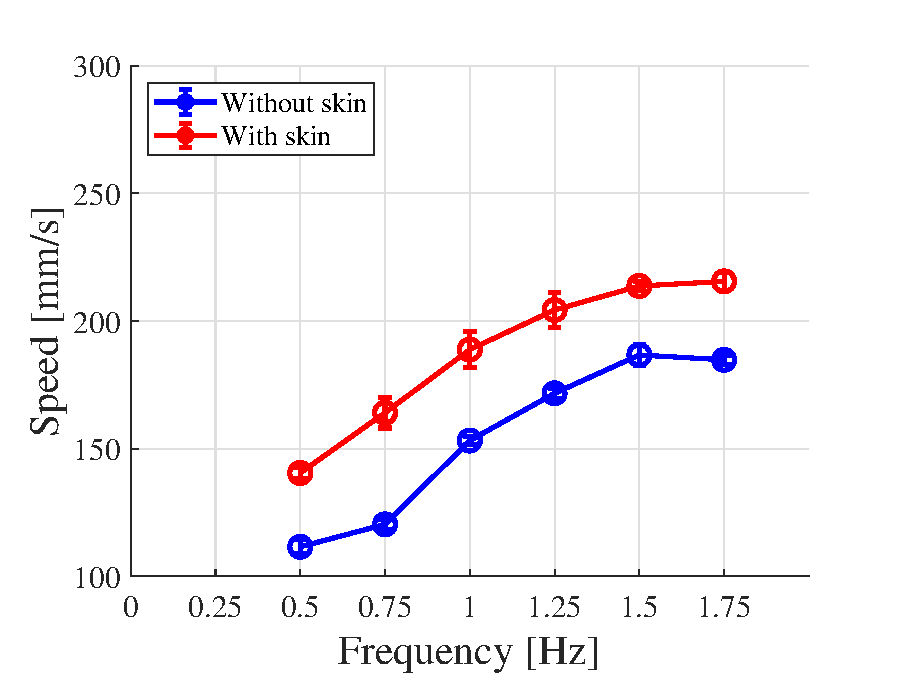
\includegraphics[width=0.9\linewidth]{chapters/picture/an90.eps}
       \subcaption{尾びれ振幅$81\:^\circ$の場合}
       \label{fig:an90}
   \end{subfigure}
   \begin{subfigure}[b]{0.53\linewidth}
       \centering
       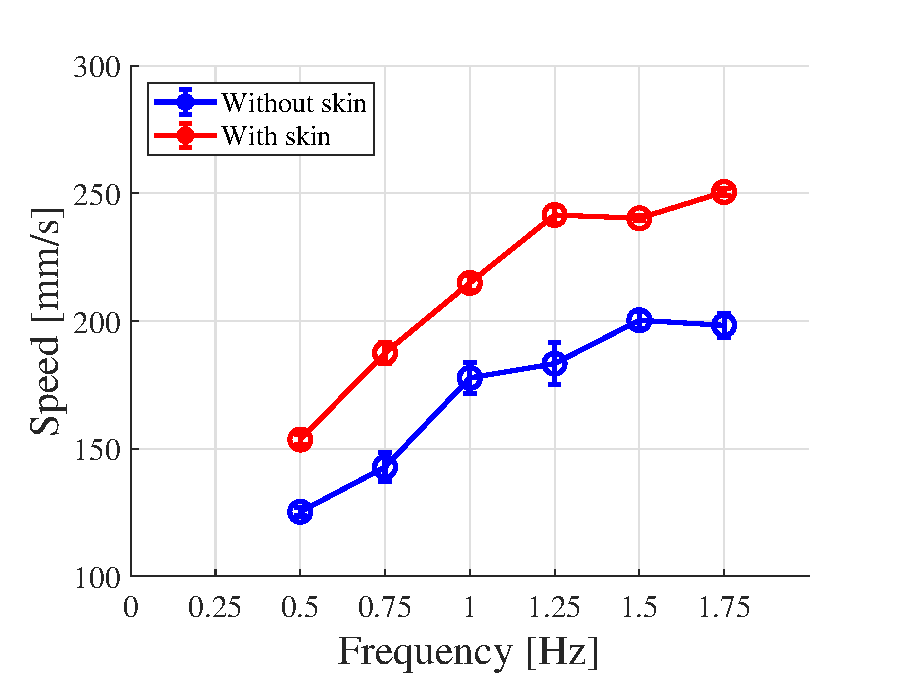
\includegraphics[width=0.9\linewidth]{chapters/picture/an135.eps}
       \subcaption{尾びれ振幅$114\:^\circ$の場合}
       \label{fig:an135}
   \end{subfigure}
   \begin{subfigure}[b]{0.53\linewidth}
       \centering
       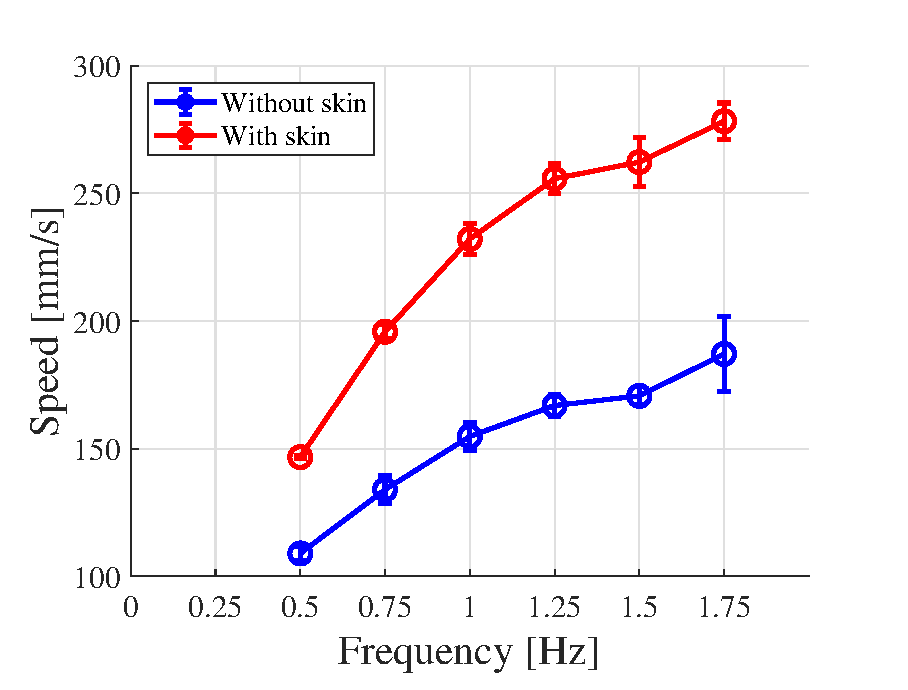
\includegraphics[width=0.9\linewidth]{chapters/picture/an180.eps}
       \subcaption{尾びれ振幅$168\:^\circ$の場合}
       \label{fig:an180}
   \end{subfigure}
   \caption{遊泳速度,尾びれ振幅および尾びれ周波数の関係}
   \label{fig:amp}
\end{figure}